251. \begin{figure}[ht!]
\center{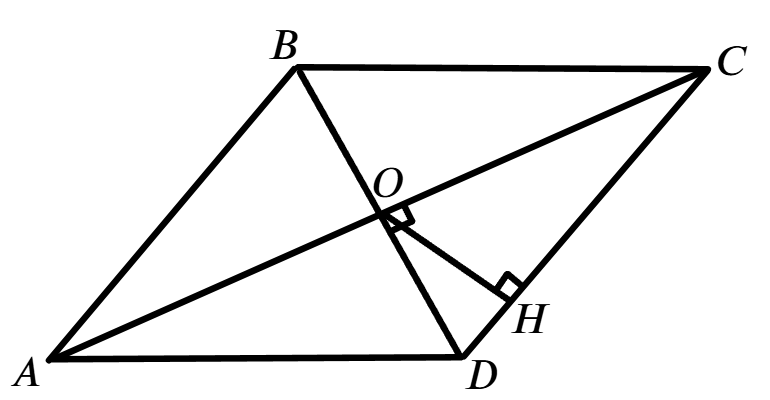
\includegraphics[scale=0.35]{g8-246.png}}
\end{figure}\\
Так как в ромбе диагонали перпендикулярны, и квадрат высоты, проведённой из прямого угла, равен произведению отрезков, на которые она делит гипотенузу, имеем соотношение $OH^2=DH\cdot4DH,\ 4=4DH^2,\ DH=1$см. Тогда по теореме Пифагора найдём диагонали (они в ромбе делятся точкой пересечения пополам):
$OD=\sqrt{1+4}=\sqrt{5},\ BD=2\sqrt{5}$см и $OC=\sqrt{16+4}=2\sqrt{5},\ AC=4\sqrt{5}$см.\\
